\chapter{Review of existing solutions}
Image Segmentation is not a new concept and is widely used in various areas such as machine vision. It is also a topic of many research papers and coding projects. While conducting research for our project, we encountered many different similar solutions both in terms of overall instance segmentation as well as essential parts of our project, like dataset preparation or raw image, point cloud and stream filtration. This chapter covers some of the solutions that we either took inspiration from or that helped us understand crucial concepts.


%=======================================
\section{DETR}
DETR \cite{carion2020endtoend} (DEtection TRansformer) approaches object detection as a direct set prediction problem. It consists of a set-based global loss, which forces unique predictions via bipartite matching, and a Transformer encoder-decoder architecture. Given a fixed small set of learned object queries, DETR reasons about the relations of the objects and the global image context to directly output the final set of predictions in parallel. Due to this parallel nature, DETR is very fast and efficient.

\begin{figure}[ht]
    \centering
    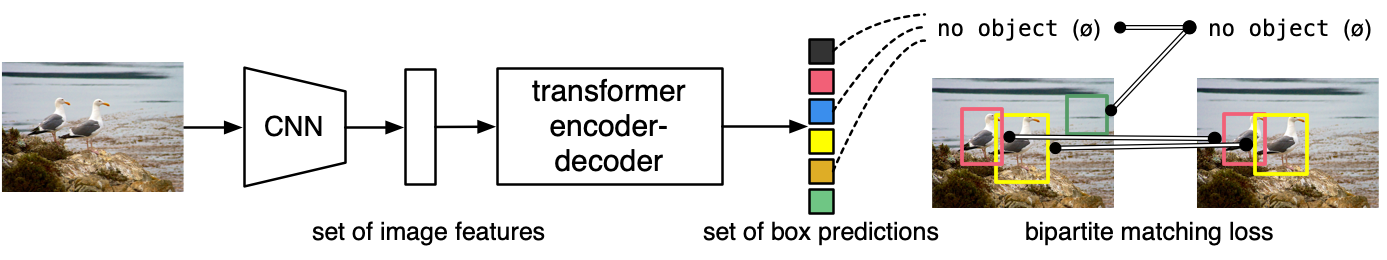
\includegraphics[width=1.0\textwidth]{img/DETR.png}
    \caption{DETR's architecture as presented in the paper \cite{carion2020endtoend}.}
    \label{fig:detr-architecture}
\end{figure}


In the first stage (\cref{fig:detr-architecture}), feature maps are extracted from the images via a Backbone layer. Many different models can be used, such as RestNet-50 or ResNet-101 \cite{he2015deep}. In this way, 2-dimensional structure information is preserved. In the following stages, the data is flattened, so we get a 1-dimensional structure. After positional encoding, it is transferred to the encoder-decoder mechanism. Finally, each output is forwarded to the Feed Forward Network.

The last layer consists of 3 nodes. The normalized center coordinates of the predicted object and the predicted height and width values of the object are obtained where the Relu activation function is used. The class of the relevant object is predicted where the softmax activation function is used in the node. Thus, there is no need for Non-Maximum Suppression (NMS).

In the Positional Encoding section, the vector of each element (or token in NLP world) is re-created according to its place in the array. Thus, the same word can have different vectors at different positions in the array.
In the encoder layer, the reduction of high-dimensional feature matrix to lower-dimensional feature matrices is performed. It consists of multi-head self attention, normalizer and feed forward network modules in each encoder layer.
In the decoder layer, there are multi-head self attention, normalizer and feed forward network modules just like the encoder. N number of object queries are converted as output embedding. In the next stage, final estimation processes are carried out with the feed forward network.



%=======================================
\section{OneFormer}
OneFormer \cite{jain2023oneformer} is a universal image segmentation framework jointly trained on the panoptic, semantic, and instance segmentation. It outperforms existing state-of-the-arts on all three image segmentation tasks, by only training once on one panoptic dataset, instead of having to be trained separately for each task. Since 2023, it is available as a part of HuggingFace's \textit{transformers} \cite{huggingface-transformers} library.

\begin{figure}[ht]
    \centering
    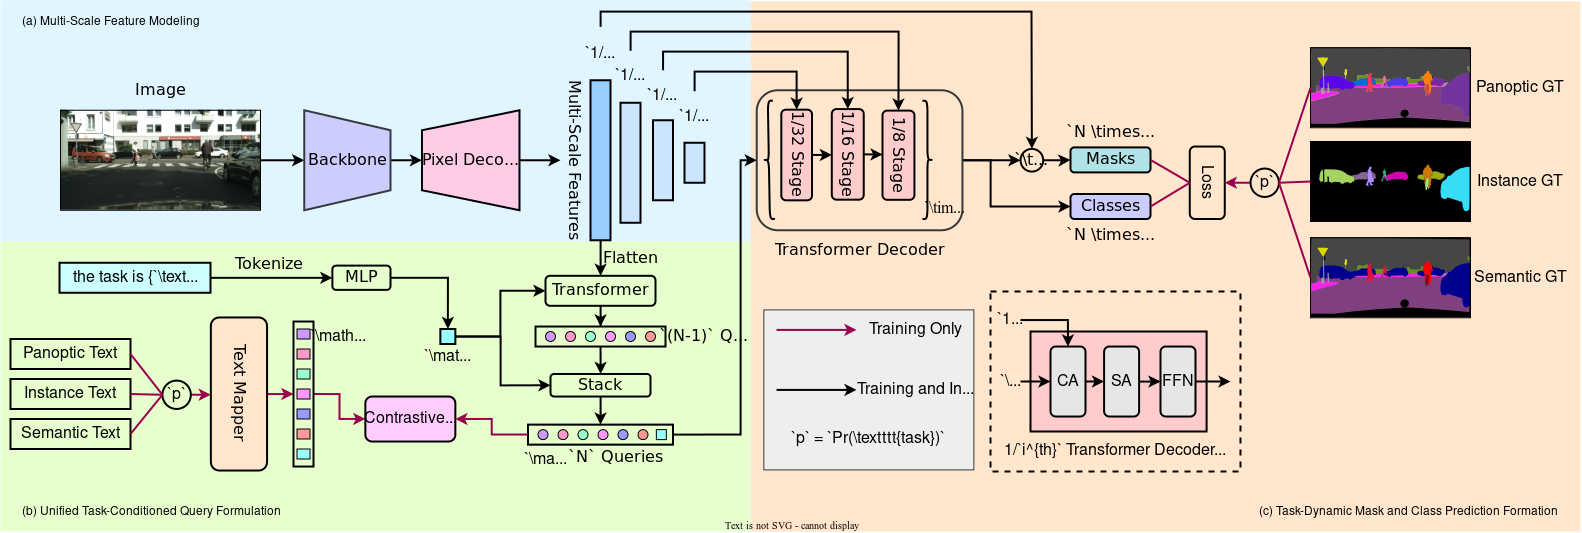
\includegraphics[width=1.0\textwidth]{img/oneformer.png}
    \caption{OneFormer's framework as presented in the paper \cite{jain2023oneformer}. The framework was implemented using Detectron2 \cite{wu2019detectron2} library. }
    \label{fig:oneformer-framework}
\end{figure}


The authors prepared a large number of pre-trained models with different backbones as well as trained and validated on different datasets, all of which can be downloaded from the project's github repository \cite{oneformer-repo}:
 
\begin{itemize}
    \item Backbones - the available models utilise commonly used backbones pretrained on the ImageNet-22K \cite{deng2009imagenet} to extract multi-scale feature representations from the input image. Then, a pixel decoder with a \textit{Multi-Scale Deformable Transformer} \cite{zhu2020deformable, cheng2021mask2former} based architecture aids the feature modeling by gradually upsampling the backbone features. The Swin-Transformer \cite{liu2021Swin}, ConvNeXt \cite{liu2022convnet}, and DiNAT \cite{hassani2022dilated} backbones were used for the experiments.
    \item Datasets - the models were trained with a batch size of 16, on three popular datasets that support the three aforementioned segmentation tasks: semantic, instance and panoptic. The datasets used are ADE20K \cite{zhou2019semantic, zhou2017scene}, CityScapes \cite{Cordts2016Cityscapes}, and COCO \cite{lin2015microsoft}.
\end{itemize}


%=======================================
\section{ISBNet}
ISBnet \cite{ngo2023isbnet} is a neural network model developed by VinAI Research, designed to tackle the task of instance segmentation, which involves identifying and delineating specific objects within an image. It leverages advanced deep learning techniques to accurately and efficiently segment objects, making it a valuable tool for computer vision applications.
To address the limitations of DyCo3D \cite{He2021dyco3d}, researchers proposed ISBNet, a cluster-free framework for 3DIS with Instance-aware Farthest Point Sampling and Box-aware Dynamic Convolution.

An auxiliary branch of the model jointly predicts the axis-aligned bounding box and the binary mask of each instance. The ground-truth axis-aligned bounding box is deduced from the existing instance mask label.

\begin{figure}[ht]
    \centering
    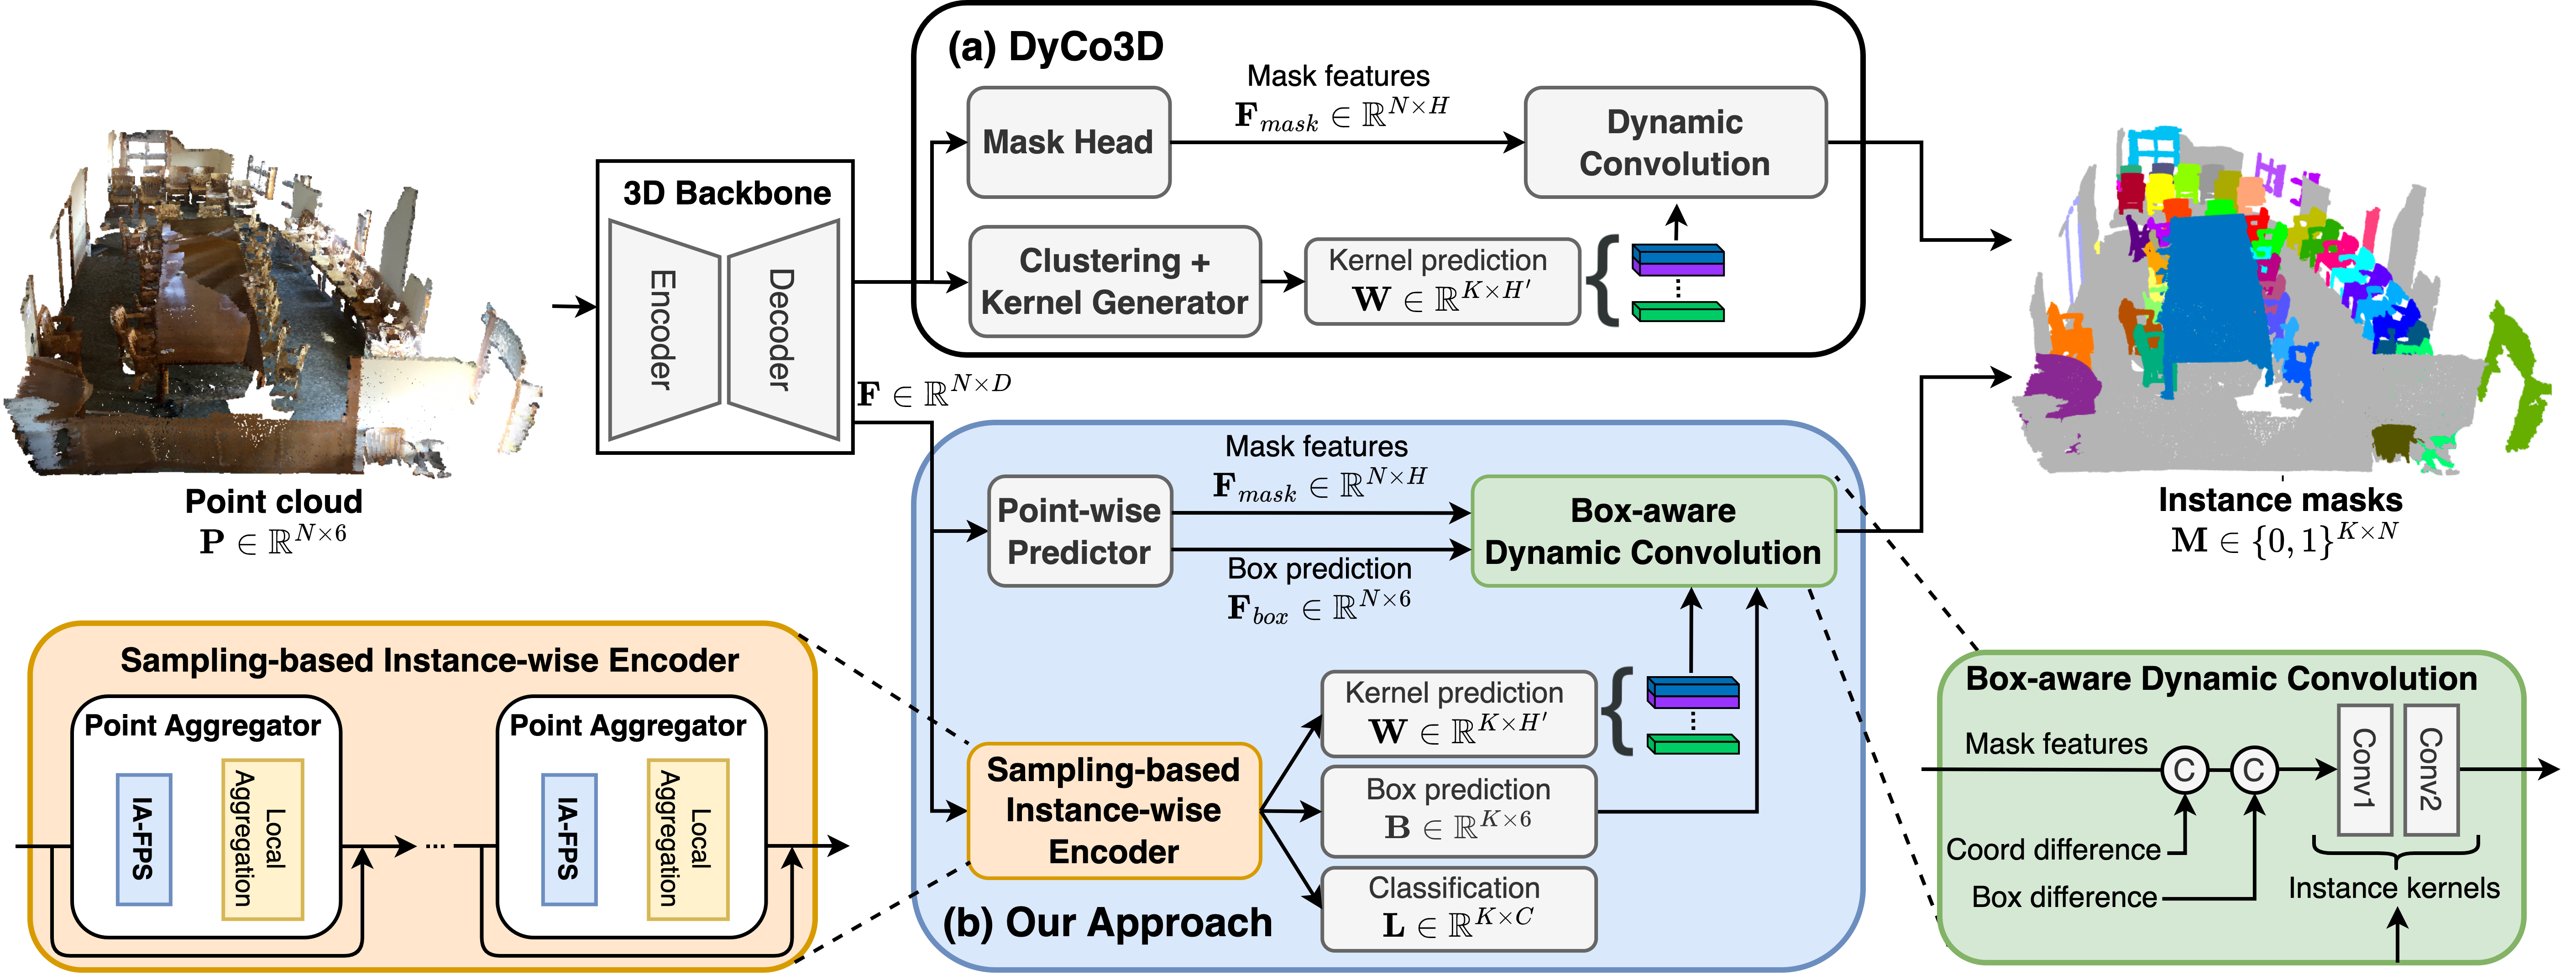
\includegraphics[width=1.0\textwidth]{img/isbnet_arch.png}
    \caption{Architectures of DyCo3D (block a) and ISBNet's approach (block b), as presented in the paper \cite{ngo2023isbnet}.}
    \label{fig:isbnet-architecture}
\end{figure}
	
Given a point cloud, a 3D backbone is employed to extract per-point features (\cref{fig:isbnet-architecture}). For DyCo3D, it first groups points into clusters based on the predicted object centroid from each point to generate a kernel for each cluster. In the meantime, the mask head transforms the per-point features into mask features for dynamic convolution. In ISBNet, the clustering algorithm is replaced with a novel sampling-based instance-wise encoder to obtain faster and more robust kernel, box, and class predictions. Furthermore, a point-wise predictor replaces the mask head of DyCo3D to output the mask and box features for a new box-aware dynamic convolution to produce more accurate instance masks.

ISBNet not only achieves the highest accuracy among these three datasets, surpassing the strongest method by +2.7/2.4/3.0 on Scan-NetV2 \cite{dai2017scannet}, S3DIS \cite{armeni2017joint}, and STPLS3D \cite{Chen_2022_BMVC}, but also demonstrates to be highly efficient, running at 237ms per scene on ScanNetV2.



%=======================================
\section{Amodal3Det}
Amodal3Det \cite{zhuo17amodal3det} is a neural network model available on GitHub and developed by the Phoenix Neural Networks team. It focuses on the challenging task of amodal 3D object detection, which involves detecting and localizing objects in 3D space, even when they are partially occluded or invisible. This model incorporates state-of-the-art techniques in deep learning and computer vision to address the complex problem of accurately detecting objects in challenging scenarios. The architecture of the Amodal3Det network is based on state-of-the-art techniques in deep learning and computer vision. 

\begin{figure}[ht]
    \centering
    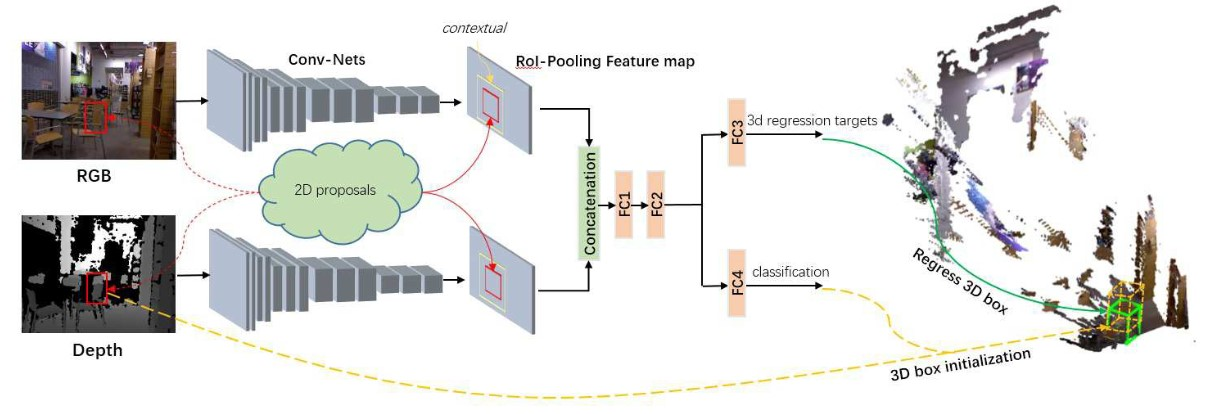
\includegraphics[width=1.0\textwidth]{img/amodal3det.jpg}
    \caption{Overview of Amodal3Det's 3D object detection system. For each 2D segment proposal, firstly the localization of a 3D box is initialized (yellow dash box) based on depth information and its size according to class wise prior knowledge. Then object class and 3D regression offsets are jointly learned based on 2D features only, with the goal of obtaining the final 3D detection (green solid box) by adjusting the location, dimension, and orientation of the initial 3D box.}
    \label{fig:amodal-arch}
\end{figure}


The labeled NYU Depth V2 \cite{Silberman:ECCV12} dataset is one of the most popular but very challenging dataset in the RGBD scene understanding research community. The original version provides 1449 RGB-Depth indoor scene images with dense 2D pixel wise class labels. To enrich the labeling features and encourage 3D object detection research, in the SUN RGBD dataset \cite{sunrgbd} (superset of NYUV2) researchers added extra 3D bounding boxes and room layouts to ground truth annotations. Since depth maps are imperfect in reality due to measurement noise, light reflection and absorption, and occlusion etc, they also refined the quality of depth maps by integrating multiple RGB-D frames from the NYUV2 raw video data.

Given a pair of color and depth images, the goal of the amodal 3D object detection is to identify the object instance locations and its full extent in 3D space. Objects that were used were a bathtub, bed, bookshelf, box, chair, counter, desk, door, dresser, garbage bin, lamp, monitor, nightstand, pillow, sink, sofa, table, tv, toilet. 

To train the Amodal3Det model, the Phoenix Neural Networks team utilized large-scale datasets specifically curated for amodal 3D object detection. These datasets would consist of 3D scenes with various objects in different poses, occlusion levels, and viewpoints. The annotations in the training data would include the 3D bounding box information for both visible and occluded parts of the objects, providing the model with the necessary supervision to learn the task effectively.



%=======================================
\section{DeepLabV3}
DeepLabV3 \cite{deeplabv3plus2018, chen2017rethinking} is a state-of-the-art deep learning model designed for semantic image segmentation. The underlying architecture of DeepLabV3 is based on a convolutional neural network (CNN) framework. The model consists of an encoder network, which extracts high-level features from the input image, and a decoder network, which generates dense pixel-level predictions.

The DeepLabV3 model takes an image as input. Following this action the input image is fed into a pre-trained CNN, such as ResNet \cite{he2015deep} or MobileNet \cite{mobilenetv32019}, which acts as the encoder network. Atrous Convolutions (dilated convolutions) are applied which increase the receptive field without reducing the spatial resolution. This allows the model to capture both local and global contextual information effectively. Next the Atrous Spatial Pyramid Pooling (ASPP) is used which involves applying atrous convolutions with different dilation rates in parallel to capture context at multiple scales. This enables the model to incorporate both fine-grained details and global context into its predictions. Then the decoder employs bilinear upsampling to increase the spatial resolution of the feature maps. Using skip connections, high-resolution future maps are combined from the encoder network with upsampled feature maps from the decoder network. This helps to preserve local information and enhance the segmentation accuracy. Finally the combined feature maps are further processed through additional convolutional layers to generate the final dense pixel-wise predictions. The output is a segmentation map, where each pixel is assigned a label corresponding to a specific object class. 

While working with DeepLabV3 we decided to create our own dataset based on the ADE20K \cite{zhou2017scene, zhou2019semantic}, which would include objects photographed in the laboratory.

